%versi 3 (22-07-2020)
\chapter{Landasan Teori}
\label{chap:teori}

Pada bab 2 ini, akan dijelaskan dasar teori terkait dengan aplikasi Rugby Indonesia saat ini, Ionic dan Capacitor. 

\section{Rugby Indonesia App}
\label{sec:skripsi} 
    Aplikasi Rugby Indonesia merupakan aplikasi resmi dari Persatuan Rugby Union Indonesia yang dapat memberikan informasi terbaru mengenai olahraga rugby di Indonesia. Aplikasi ini dapat memberikan notifikasi langsung mengenai berita terakhir, turnamen yang akan datang, dan informasi lainnya. Selain itu, aplikasi ini juga memungkinkan pengguna untuk mengambil gambar dan menunjukkan dukungan mereka dengan rekan-rekan penggemar rugby lainnya. Terdapat juga aplikasi multimedia pengenalan olahraga rugby berbasis Android yang dapat memberikan informasi sejarah, peraturan, dan peralatan serta tempat-latihan rugby di beberapa Kabupaten/Kota. Aplikasi Rugby Indonesia tersedia di Google Play Store dan dapat diunduh secara gratis.

    \begin{figure} [!h]
        \centering
        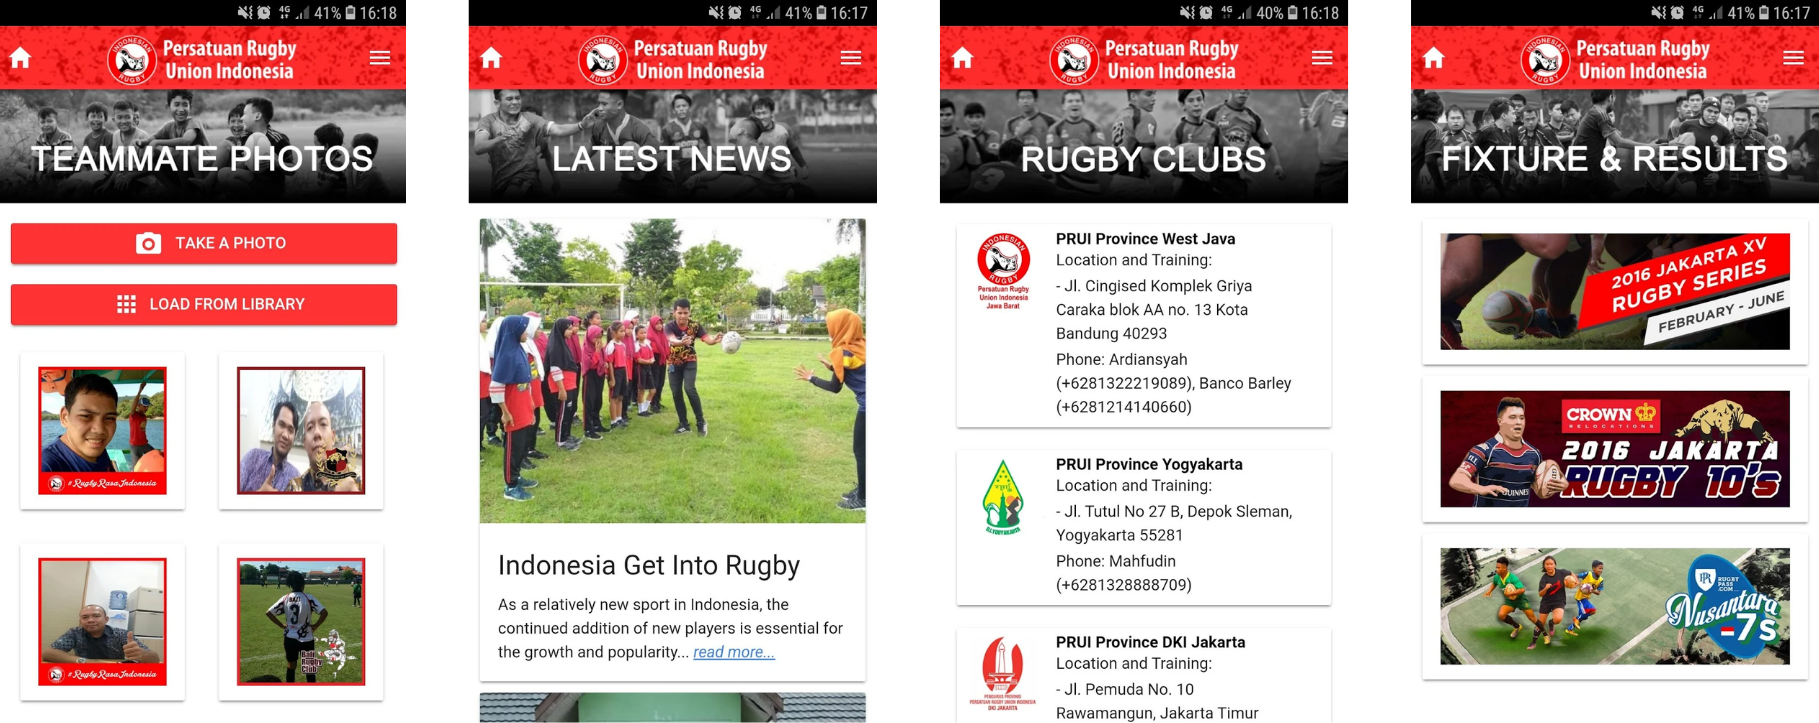
\includegraphics[scale=0.725]{Gambar/Rugby-Indonesia-App-UI.png}
        \caption[Halaman aplikasi Rugby Indonesia]{Halaman-halaman dari aplikasi Rugby Indonesia}
        \label{fig:halaman-rugby-indonesia}
    \end{figure}

    Fitur-fitur yang ada pada aplikasi Rugby Indonesia saat ini yaitu:

    \begin{enumerate}
        \item Halaman \textit{Latest News} yang diambil dari \url{https://rugbyindonesia.or.id/berita/} dengan memanfaatkan protokol RSS.
        \item Halaman \textit{Fixture \& Results}.
        \item Halaman \textit{Teammate Photos} dengan fungsi:
        \begin{itemize}
            \item Pengguna dapat langsung mengambil foto dari aplikasi tersebut.
            \item Pengguna dapat langsung memberikan \textit{frame} terhadap foto tersebut.
            \item Pengguna dapat langsung menggunggah foto tersebut ke dalam galeri publik.
        \end{itemize}
    \item Halaman \textit{Rugby Clubs} yang memiliki fungsi di mana pengguna dapat langsung mendaftar ke dalam \textit{Rugby Clubs} yang berada di Indonesia.
    \item Fungsi \textit{Push Notifications}.
    \end{enumerate}
% Rencananya akan diisi dengan penjelasan umum mengenai buku skripsi.

% \dtext{11-12} 

% \section{\LaTeX}
\section{ReactJS}
\label{sec:latex}

% Mengapa menggunakan \LaTeX{} untuk buku skripsi dan apa keunggulan/kerugiannya bagi mahasiswa dan pembuat template. 

% \dtext{13-14}

ReactJS atau React adalah sebuah library JavaScript yang digunakan untuk membangun user interface yang interaktif. ReactJS berisi kumpulan snippet kode JavaScript yang disebut "komponen" yang bisa digunakan berulang kali untuk mendesain antarmuka pengguna. ReactJS bukanlah framework JavaScript, karena hanya bertugas untuk merender komponen area tampilan aplikasi. ReactJS dapat digunakan untuk membuat aplikasi web dan mobile.

React dibuat oleh Jordan Walke, seorang insinyur perangkat lunak di Facebook (sekarang bernama Meta), yang merilis prototipe awal React yang disebut ``FaxJS''. Dia terinspirasi dari bahasa pemrograman XHP, perpustakaan komponen HTML untuk PHP. React pertama kali diterapkan di Facebook's News Feed pada tahun 2011 dan kemudian di Instagram pada tahun 2012. React bersifat open-source di JSConf US pada Mei 2013.

Beberapa fitur dan kelebihan ReactJS antara lain:

\begin{itemize}
    \item Reusable Components: Dengan ReactJS, Anda bisa menggunakan lagi komponen yang sudah dikembangkan menjadi aplikasi. Sebab, ReactJS adalah library yang open-source, sehingga Anda bisa membangun komponen siap pakai, yang akan mempercepat proses development aplikasi web kompleks.
    \item Virtual DOM: ReactJS menggunakan Virtual DOM, yang memungkinkan perubahan pada tampilan aplikasi hanya terjadi pada bagian yang berubah saja, tanpa harus merender ulang seluruh tampilan aplikasi. Hal ini membuat aplikasi menjadi lebih cepat dan efisien.
    \item SEO-Friendly: ReactJS bisa memaksimalkan optimisasi mesin pencari (SEO) aplikasi web dengan meningkatkan performanya. Sebab, implementasi Virtual DOM merupakan salah satu faktor yang memengaruhi kecepatan.
    \item Learn Once, Write Anywhere: ReactJS tidak membuat asumsi tentang sisa stack pengguna, sehingga pengguna dapat mengembangkan fitur baru di React tanpa menulis ulang kode yang ada. React juga dapat me-render di server dengan menggunakan Node dan menjalankan aplikasi seluler menggunakan React Native.
    \item UI Interaktif: ReactJS dapat disebut sebagai “Learn One – Write Anywhere” library, karena baik dalam pengembangan aplikasi web dan mobile, React mengikuti pola desain yang sama, memfasilitasi proses transisi. Menggunakan JavaScript polos dan React, Anda dapat membuat UI yang kaya untuk aplikasi asli, serta didukung oleh platform iOS dan Android. 
\end{itemize}

Dengan kelebihan-kelebihan tersebut, ReactJS menjadi pilihan yang masuk akal baik untuk startup maupun perusahaan.

\section{Ionic 7 Framework}
\label{sec:template}
 
% Akan dipaparkan bagaimana menggunakan template ini, termasuk petunjuk singkat membuat referensi, gambar dan tabel.
% Juga hal-hal lain yang belum terpikir sampai saat ini. 
 
% \dtext{15/-16}

Ionic 7 adalah sebuah framework untuk membangun aplikasi mobile hybrid menggunakan HTML5, CSS, dan AngularJS. Framework ini dirilis pada tanggal 29 Maret 2023 dan memiliki beberapa perbaikan yang diusulkan oleh komunitas Ionic. Beberapa fitur baru di Ionic 7 antara lain:

\begin{itemize}
    \item Inline Overlays: Cara yang lebih efisien untuk bekerja dengan form-control seperti Toggle atau Input. Komponen Item dan Label tidak lagi diperlukan, dan setiap form-control menangani konten label secara langsung. Perubahan ini mengurangi boilerplate kode dengan menghilangkan persyaratan ion-item dan ion-label.
    \item Performa yang Lebih Baik: Ionic 7 secara signifikan meningkatkan performa Tabs. Pada Ionic React dan Ionic Vue, pengembang dapat mengharapkan peningkatan performa hingga 70\% saat beralih tab. Pengembang Ionic Angular dapat mengharapkan waktu inisialisasi komponen Ionic yang lebih baik berkat optimasi di Stencil.
    \item Kompatibilitas Vite yang Lebih Baik: Ionic 7 menghapus titik masuk Common JS untuk Ionic React dan Ionic Vue untuk membuat setiap paket lebih mudah digunakan dengan Vite dan Vitest.
\end{itemize}
Ionic 7 mendukung Angular 14+, React 17+, dan Vue 3.0.6+.

\subsection{UI Components}
UI Components pada Ionic 7 adalah kumpulan komponen yang digunakan untuk membangun antarmuka pengguna aplikasi mobile hybrid. Komponen-komponen ini memungkinkan pengembang untuk dengan cepat membangun antarmuka pengguna yang menarik dan responsif. Komponen yang terdapat pada Ionic 7 yaitu:

\subsubsection{Action Sheet}
Action Sheet (ion-action-sheet) merupakan sebuah komponen yang berguna untuk memunculkan dialog. Dialog tersebut akan melakukan pemberhentian sementara terhadap aplikasi yang sedang dijalankannya dan pengguna harus memilih pilihan yang berada di dalam dialog tersebut. Cara penggunaan dari Action Sheet adalah sebagai berikut:

\begin{lstlisting}[language=HTML, caption=Contoh kode untuk membuat Action Sheet, label=kode:ion-action-sheet]
import React from 'react';
import { IonActionSheet, IonButton } from '@ionic/react';

function Example() {
  return (
    <>
      <IonButton id="open-action-sheet">Open</IonButton>
      <IonActionSheet
        trigger="open-action-sheet"
        header="Actions"
        buttons={[
          {
            text: 'Delete',
            role: 'destructive',
            data: {
              action: 'delete',
            },
          },
          {
            text: 'Share',
            data: {
              action: 'share',
            },
          },
          {
            text: 'Cancel',
            role: 'cancel',
            data: {
              action: 'cancel',
            },
          },
        ]}
      ></IonActionSheet>
    </>
  );
}
export default Example;
\end{lstlisting}

\subsubsection{Accordion}
Accordion berfungsi untuk mengurangi ruang vertikal dalam mengorganisir informasi yang ingin ditampilkan. Accordion memiliki 2 komponen yaitu ion-accordion dan ion-accordion-group. Ketika menggunakan accordion, ion-accordion harus berada di dalam ion-accordion-group. Contoh penggunaan dari Accordion adalah sebagai berikut:

\begin{lstlisting}[language=HTML, caption=Contoh kode untuk membuat Accordion, label=kode:ion-accordion]
import React from 'react';
import { IonAccordion, IonAccordionGroup, IonItem, IonLabel } from '@ionic/react';
function Example() {
  return (
    <IonAccordionGroup>
      <IonAccordion value="first">
        <IonItem slot="header" color="light">
          <IonLabel>First Accordion</IonLabel>
        </IonItem>
        <div className="ion-padding" slot="content">
          First Content
        </div>
      </IonAccordion>
      <IonAccordion value="second">
        <IonItem slot="header" color="light">
          <IonLabel>Second Accordion</IonLabel>
        </IonItem>
        <div className="ion-padding" slot="content">
          Second Content
        </div>
      </IonAccordion>
      <IonAccordion value="third">
        <IonItem slot="header" color="light">
          <IonLabel>Third Accordion</IonLabel>
        </IonItem>
        <div className="ion-padding" slot="content">
          Third Content
        </div>
      </IonAccordion>
    </IonAccordionGroup>
  );
}
export default Example;
\end{lstlisting}

\subsubsection{Alert}
Alert pada Ionic berfungsi untuk memberikan informasi serta mengumpulkan informasi dari pengguna menggunakan input dari pengguna. Sama seperti Action Sheet, Alert juga biasanya dimunculkan di atas konten dari aplikasi, namun Alert biasanya berada di tengah konten aplikasi, sedangkan Action Sheet muncul berada dari bawah aplikasi. Contoh dari penggunaan Alert adalah sebagai berikut:

\begin{lstlisting}[language=HTML, caption=Contoh kode untuk membuat Alert, label=kode:ion-alert]
import React from 'react';
import { IonAlert, IonButton } from '@ionic/react';

function Example() {
  return (
    <>
      <IonButton id="present-alert">Click Me</IonButton>
      <IonAlert
        trigger="present-alert"
        header="A Short Title Is Best"
        subHeader="A Sub Header Is Optional"
        message="A message should be a short, complete sentence."
        buttons={['Action']}
      ></IonAlert>
    </>
  );
}
export default Example;
\end{lstlisting}

\subsubsection{Badge}
Badge adalah elemen inline yang umumnya muncul di dekat dengan elemen lain. Badge ini umumnya mengandung angka atau karakter lainnya dan dapat digunakan sebagai elemen widget yang menampilkan informasi tambahan tentang elemen induk.Contoh dari penggunaan Badge adalah sebagai berikut:

\begin{lstlisting}[language=HTML, caption=Contoh kode untuk membuat Badge, label=kode:ion-badge]
<IonBadge>11</IonBadge>
\end{lstlisting}

\subsubsection{Breadcrumb}
Breadcrumb pada Ionic 7 adalah sebuah elemen navigasi tunggal yang merupakan anak dari komponen Breadcrumbs. Breadcrumb dapat berupa tautan ke tempat lain dalam aplikasi atau berupa teks biasa. Setiap breadcrumb memiliki pemisah di antara mereka dan dapat opsionalnya berisi ikon. Breadcrumb digunakan untuk menunjukkan posisi pengguna dalam aplikasi atau situs yang besar dan memiliki halaman yang tersusun secara hierarkis. Mereka dapat diklik untuk menampilkan popover dengan informasi lebih lanjut atau memperluas breadcrumb yang terlipat. Breadcrumb dapat dikonfigurasi dengan berbagai cara, seperti menambahkan ikon, mengatur jumlah maksimum item yang ditampilkan, dan mengontrol tampilan item sebelum dan setelah penggulungan. Contoh dari penggunaan Breadcrumb adalah sebagai berikut:

\begin{lstlisting}[language=HTML, caption=Contoh kode untuk membuat Breadcrumb, label=kode:ion-breadcrumb]
import React from 'react';
import { IonBreadcrumb, IonBreadcrumbs } from '@ionic/react';
function Example() {
  return (
    <IonBreadcrumbs>
      <IonBreadcrumb href="#home">Home</IonBreadcrumb>
      <IonBreadcrumb href="#electronics">Electronics</IonBreadcrumb>
      <IonBreadcrumb href="#cameras">Cameras</IonBreadcrumb>
      <IonBreadcrumb href="#film">Film</IonBreadcrumb>
    </IonBreadcrumbs>
  );
}
export default Example;
\end{lstlisting}

\subsubsection{Button}
Button merupakan elemen interaktif yang dapat digunakan dalam berbagai aplikasi untuk menyediakan fitur tombol standar. Berikut adalah contoh dari penggunaan Button:

\begin{lstlisting}[language=HTML, caption=Contoh kode untuk membuat Button, label=kode:ion-button]
<IonButton>Default</IonButton>
\end{lstlisting}

\subsubsection{Card}
Card merupakan komponen UI yang digunakan untuk menampilkan konten seperti teks, gambar, tombol, dan daftar dalam sebuah kotak. Komponen ini biasanya terdiri dari header, judul, gambar, dan konten utama. Card dapat digunakan sebagai komponen tunggal atau digabungkan dengan komponen lain untuk membuat tampilan yang lebih kompleks. Card dapat disesuaikan dengan menggunakan properti CSS seperti background dan color. Berikut merupakan contoh dari penggunaan Card:

\begin{lstlisting}[language=HTML, caption=Contoh kode untuk membuat Card, label=kode:ion-card]
import React from 'react';
import { IonCard, IonCardContent, IonCardHeader, IonCardSubtitle, IonCardTitle } from '@ionic/react';

function Example() {
  return (
    <IonCard>
      <IonCardHeader>
        <IonCardTitle>Card Title</IonCardTitle>
        <IonCardSubtitle>Card Subtitle</IonCardSubtitle>
      </IonCardHeader>

      <IonCardContent>Here's a small text description for the card content. Nothing more, nothing less.</IonCardContent>
    </IonCard>
  );
}
export default Example;
\end{lstlisting}

\subsubsection{Checkbox}
Checkbox merupakan komponen yang memungkinkan pengguna untuk memilih beberapa opsi dari satu set dan muncul sebagai dicentang ketika diaktifkan. Komponen ini digunakan dengan tag <ion-checkbox>. Contoh dari penggunaan Checkbox adalah sebagai berikut:

\begin{lstlisting}[language=HTML, caption=Contoh kode untuk membuat Checkbox, label=kode:ion-checkbox]
<IonCheckbox>I agree to the terms and conditions</IonCheckbox>
\end{lstlisting}

\subsubsection{Chip}
Chip pada Ionic 7 adalah elemen yang digunakan untuk menampilkan informasi dalam bentuk container kecil, seperti bubuk. Chip ini dapat berisi berbagai elemen seperti avatar, teks, dan ikon. Contohdari penggunaan Chip adalah sebagai berikut:

\begin{lstlisting}[language=HTML, caption=Contoh kode untuk membuat Button, label=kode:ion-chip]
import React from 'react';
import { IonChip } from '@ionic/react';
function Example() {
  return (
    <>
      <IonChip>Default</IonChip>
      <IonChip disabled={true}>Disabled</IonChip>
      <IonChip outline={true}>Outline</IonChip>
    </>
  );
}
export default Example;
\end{lstlisting}

\subsubsection{Content}
Content merupakan komponen yang berguna untuk menyediakan area konten yang dapat dikontrol dan diubah menggunakan CSS. Dalam satu tampilan hanya terdapat satu konten. Konten dan komponen Ionic lainnya dapat dikostumisasi ulang dengan menggunakan CSS yang tersedia. Berikut adalah contoh dari penggunaan Content:

\begin{lstlisting}[language=HTML, caption=Contoh kode untuk membuat Content, label=kode:ion-content]
import React from 'react';
import { IonContent } from '@ionic/react';

function Example() {
  return (
    <IonContent className="ion-padding">
      <h1>Heading 1</h1>

      <p>Here's a small text description for the content. Nothing more, nothing less.</p>
    </IonContent>
  );
}
export default Example;
\end{lstlisting}

\subsubsection{Toolbar}
Toolbar merupakan komponen yang digunakan untuk menampilkan judul, tombol, ikon, tombol kembali, tombol menu, kotak pencarian, segmen, dan indikator progres di aplikasi. Toolbars umumnya ditempatkan di atas atau di bawah konten dan menyediakan konten dan tindakan untuk layar saat ini. Ketika toolbar ditempatkan di header, toolbar akan muncul di bagian atas konten, sedangkan jika ditempatkan di footer, toolbar akan muncul di bagian bawah. Berikut adalah contoh penggunaan Toolbar:

\begin{lstlisting}[language=HTML, caption=Contoh kode untuk membuat Toolbar, label=kode:ion-toolbar]
import React from 'react';
import { IonFooter, IonHeader, IonTitle, IonToolbar } from '@ionic/react';

function Example() {
  return (
    <>
      <IonHeader>
        <IonToolbar>
          <IonTitle>Header Toolbar</IonTitle>
        </IonToolbar>
      </IonHeader>

      <IonFooter>
        <IonToolbar>
          <IonTitle>Footer Toolbar</IonTitle>
        </IonToolbar>
      </IonFooter>
    </>
  );
}
export default Example;
\end{lstlisting}

\subsection{Capacitor Native}
Native merupakan kemampuan untuk menambahkan fungsionalitas perangkat asli ke dalam aplikasi menggunakan plugin API untuk Swift pada iOS, Java pada Android, dan JavaScript untuk web. Dengan menggunakan plugin ini, pengembang dapat membuat pengalaman "native" yang disesuaikan dengan mudah. Ionic menyediakan Capacitoe sebagai sebuah runtime native yang memungkinkan menambahkan fungsionalitas perangkat asli ke dalam aplikasi.

Pengembang yang menggunakan Capacitor harus menginstal capacitor tersebut terlebih dahulu dengan cara:
\begin{lstlisting}[language=HTML, caption=Kode untuk menginstal Capacitor Camera, label=kode:install-capacitor]
$ npm install @capacitor/camera
\end{lstlisting}

Berikut cara menggunakan Capacitor dengan menggunakan plugin Camera:

\begin{lstlisting}[language=HTML, caption=Contoh kode Capacitor, label=kode:capacitor-camera-example]
import { Camera, CameraResultType } from '@capacitor/camera';

const takePicture = async () => {
  const image = await Camera.getPhoto({
    quality: 90,
    allowEditing: true,
    resultType: CameraResultType.Uri
  });
  const imageUrl = image.webPath;
  imageElement.src = imageUrl;
};
\end{lstlisting}

\subsubsection{Action Sheet}

Action Sheet merupakan sebuah dialog yang menampilkan serangkaian opsi di atas konten aplikasi dan harus ditutup secara manual oleh pengguna sebelum mereka dapat melanjutkan interaksi dengan aplikasi. Opsi yang merusak dibuat jelas dalam mode ios. Ada beberapa cara untuk menutup action-sheet, termasuk mengetuk latar belakang atau menekan tombol escape di desktop. Action-sheet dapat dikendalikan menggunakan properti isOpen untuk mengontrol status presentasi dari Action Sheet dari state aplikasi. Action-sheet juga memiliki properti seperti header untuk judul, buttons untuk menambahkan tombol, dan keyboardClose untuk menutup action-sheet ketika tombol keyboard tertentu ditekan. Berikut cara menginstall Action Sheet:

\begin{lstlisting}[language=HTML, caption=Kode untuk menginstal Plugin Action Sheet, label=kode:install-action-sheet-capacitor]
npm install @capacitor/action-sheet
\end{lstlisting}

Berikut merupakan contoh dari penggunaan Action Sheet:

\begin{lstlisting}[language=HTML, caption=Contoh kode plugin Action Sheet, label=kode:capacitor-action-sheet-example]
import { ActionSheet, ActionSheetButtonStyle } from '@capacitor/action-sheet';

const showActions = async () => {
  const result = await ActionSheet.showActions({
    title: 'Photo Options',
    message: 'Select an option to perform',
    options: [
      {
        title: 'Upload',
      },
      {
        title: 'Share',
      },
      {
        title: 'Remove',
        style: ActionSheetButtonStyle.Destructive,
      },
    ],
  });

  console.log('Action Sheet result:', result);
};
\end{lstlisting}

\subsubsection{Camera}
Plugin Camera pada Ionic 7 adalah sebuah plugin yang memungkinkan pengguna untuk mengambil foto dengan kamera atau memilih foto yang sudah ada dari album foto. Plugin ini dapat diinstal dengan perintah npm install @capacitor/camera dan npx cap sync untuk platform iOS, serta menambahkan beberapa izin pada file Info.plist untuk iOS dan AndroidManifest.xml untuk Android. Selain itu, plugin ini juga memerlukan PWA Elements agar dapat berfungsi. Berikut merupakan contoh kode dari penggunaan Camera Plugin:

\begin{lstlisting}[language=HTML, caption=Contoh kode Capacitor Camera, label=kode:capacitor-cam-example]
import { Camera, CameraResultType } from '@capacitor/camera';

const takePicture = async () => {
  const image = await Camera.getPhoto({
    quality: 90,
    allowEditing: true,
    resultType: CameraResultType.Uri
  });

  // image.webPath will contain a path that can be set as an image src.
  // You can access the original file using image.path, which can be
  // passed to the Filesystem API to read the raw data of the image,
  // if desired (or pass resultType: CameraResultType.Base64 to getPhoto)
  var imageUrl = image.webPath;

  // Can be set to the src of an image now
  imageElement.src = imageUrl;
};
\end{lstlisting}

\subsubsection{Filesyatem}
Filesystem API menyediakan alat NodeJS-like untuk bekerja dengan file pada perangkat. Pengembang dapat menggunakan plugin ini untuk melakukan operasi file umum seperti membaca, tulis, dan mengelola isi direktori.

Berikut kode untuk menginstall Filesystem:

\begin{lstlisting}[language=HTML, caption=Kode untuk menginstal plugin Filesystem, label=kode:install-filesystem-capacitor]
npm install @capacitor/action-sheet
\end{lstlisting}

Berikut contoh penggunaan Filesystem Plugin:
\begin{lstlisting}[language=HTML, caption=Contoh kode dari penggunaan Filesystem, label=kode:example-of-filesystem-capacitor]
import { Filesystem, Directory, Encoding } from '@capacitor/filesystem';

const writeSecretFile = async () => {
  await Filesystem.writeFile({
    path: 'secrets/text.txt',
    data: 'This is a test',
    directory: Directory.Documents,
    encoding: Encoding.UTF8,
  });
};

const readSecretFile = async () => {
  const contents = await Filesystem.readFile({
    path: 'secrets/text.txt',
    directory: Directory.Documents,
    encoding: Encoding.UTF8,
  });

  console.log('secrets:', contents);
};

const deleteSecretFile = async () => {
  await Filesystem.deleteFile({
    path: 'secrets/text.txt',
    directory: Directory.Documents,
  });
};

const readFilePath = async () => {
  // Here's an example of reading a file with a full file path. Use this to
  // read binary data (base64 encoded) from plugins that return File URIs, such as
  // the Camera.
  const contents = await Filesystem.readFile({
    path: 'file:///var/mobile/Containers/Data/Application/22A433FD-D82D-4989-8BE6-9FC49DEA20BB/Documents/text.txt',
  });

  console.log('data:', contents);
};
\end{lstlisting}

\subsubsection{Preference}
Plugin Preference pada Ionic 7 adalah alat yang memungkinkan Anda untuk menyimpan data sederhana dalam bentuk kunci/nilai yang dapat diakses secara bersamaan. Preferences API menyediakan area penyimpanan data yang mendukung kunci/nilai untuk aplikasi Ionic. Beberapa fitur utama dari Plugin Preference meliputi:
\begin{itemize}
    \item Mengatur grup preferences: Preferences grups digunakan untuk mengatur kunci/nilai pairs. Menggunakan nilai 'NativeStorage' memberikan kompatibilitas belakang dengan cordova-plugin-nativestorage.
    \item Mengakses hasil preferences: Menggunakan getResult() method sehingga mendapatkan nilai dari preferences yang terkait dengan kunci tertentu
    \item Menyimpan dan mengatur preferences: Menggunakan metode set() untuk menyimpan atau mengatur nilai preferences
\end{itemize}

Untuk menggunakan Plugin Preference dalam aplikasi Ionic, perlu menginstal plugin Capacitor Preferences dengan cara:

\begin{lstlisting}[language=HTML, caption=Kode untuk menginstal plugin Preference, label=kode:install-preference-capacitor]
npm install @capacitor/preferences
\end{lstlisting}

Berikut merupakan contoh kode dari penggunaan Preference:

\begin{lstlisting}[language=HTML, caption=Contoh kode dari plugin Preference, label=kode:preference-capacitor-example]
import { Preferences } from '@capacitor/preferences';

const setName = async () => {
  await Preferences.set({
    key: 'name',
    value: 'Max',
  });
};

const checkName = async () => {
  const { value } = await Preferences.get({ key: 'name' });

  console.log(`Hello ${value}!`);
};

const removeName = async () => {
  await Preferences.remove({ key: 'name' });
};
\end{lstlisting}

% \subsection{Tabel}  
% Berikut adalah contoh pembuatan tabel. 
% Penempatan tabel dan gambar secara umum diatur secara otomatis oleh \LaTeX{}, perhatikan contoh di file bab2.tex untuk melihat bagaimana cara memaksa tabel ditempatkan sesuai keinginan kita.

% Perhatikan bawa berbeda dengan penempatan judul gambar gambar, keterangan tabel harus diletakkan di atas tabel!!
% Lihat Tabel~\ref{tab:contoh1} berikut ini:

% \begin{table}[H] %atau h saja untuk "kira kira di sini"
% 	\centering 
% 	\caption{Tabel contoh}
% 	\label{tab:contoh1}
% 	\begin{tabular}{cccc}
% 		\toprule
% 		& $v_{start}$ & $\mathcal{S}_{1}$ & $v_{end}$\\

% 		\midrule
% 		$\tau_{1}$ & 1 & 12& 20\\
% 		$\tau_{2}$ & 1 &  & 20\\
% 		$\tau_{3}$ & 1 & 9 & 20\\
% 		$\tau_{4}$ & 1 &  & 20\\

% 		\bottomrule
		
% 	\end{tabular} 
% \end{table}
% Tabel~\ref{tab:cthwarna1} dan Tabel~\ref{tab:cthwarna2} berikut ini adalah tabel dengan sel yang berwarna dan ada dua tabel yang bersebelahan. 
% \begin{table}[H]
% 	\begin{minipage}[c]{0.49\linewidth}
% 		\centering
% 		\caption{Tabel bewarna(1)}
% 		\label{tab:cthwarna1}
% 		\begin{tabular}{ccccc}
% 			\toprule
% 			 & $v_{start}$ & $\mathcal{S}_{2}$ & $\mathcal{S}_{1}$ & $v_{end}$\\
			
% 			\midrule
% 			$\tau_{1}$ & 1 & 5 \cellcolor{green}& 12& 20\\
% 			$\tau_{2}$ & 1 & 8 \cellcolor{green}& & 20\\
% 			$\tau_{3}$ & 1 & 2/8/17 \cellcolor{green}& 9 & 20\\
% 			$\tau_{4}$ & 1 & \cellcolor{red}& & 20\\
			
% 			\bottomrule

% 		\end{tabular}
% 	\end{minipage}
% 	\begin{minipage}[c]{0.49\linewidth}
		
% 		\centering 
% 		\caption{Tabel bewarna(2)}
% 		\label{tab:cthwarna2}
% 		\begin{tabular}{ccccc}
% 			\toprule
% 			 & $v_{start}$ & $\mathcal{S}_{1}$ & $\mathcal{S}_{2}$ & $v_{end}$\\
			
% 			\midrule
% 			$\tau_{1}$ & 1 & 12& 5 \cellcolor{red} &20\\
% 			$\tau_{2}$ & 1 &  &  8 \cellcolor{green} &20\\
% 			$\tau_{3}$ & 1 & 9 & 2/8/17 \cellcolor{green} &20\\
% 			$\tau_{4}$ & 1 &   & \cellcolor{red} &20\\
			
% 			\bottomrule
		
% 		\end{tabular}
% 	\end{minipage}
% \end{table}

 
% \subsection{Kutipan}
% \label{subs:kutipan} 
% Berikut contoh kutipan dari berbagai sumber, untuk keterangan lebih lengkap, silahkan membaca file referensi.bib yang disediakan juga di template ini.
% Contoh kutipan:
% \begin{itemize}
% 	\item Buku:~\cite{berg:08:compgeom} 
% 	\item Bab dalam buku:~\cite{kreveld:04:GIS}
% 	\item Artikel dari Jurnal:~\cite{buchin:13:median}
% 	\item Artikel dari prosiding seminar/konferensi:~\cite{kreveld:11:median}
% 	\item Skripsi/Thesis/Disertasi:~\cite{lionov:02:animasi}~\cite{wiratma:10:following}~\cite{wiratma:22:later}
% 	\item Technical/Scientific Report:~\cite{kreveld:07:watertight}
% 	\item RFC (Request For Comments):~\cite{RFC1654}
% 	\item Technical Documentation/Technical Manual:~\cite{Z.500}~\cite{unicode:16:stdv9}~\cite{google:16:and7}
% 	\item Paten:~\cite{webb:12:comm}
% 	\item Tidak dipublikasikan:~\cite{wiratma:09:median}~\cite{lionov:11:cpoly}
% 	\item Laman web:~\cite{erickson:03:cgmodel}  
% 	\item Lain-lain:~\cite{agung:12:tango}
% \end{itemize}    
  
% \subsection{Gambar}

% Pada hampir semua editor, penempatan gambar di dalam dokumen \LaTeX{} tidak dapat dilakukan melalui proses {\it drag and drop}.
% Perhatikan contoh pada file bab2.tex untuk melihat bagaimana cara menempatkan gambar.
% Beberapa hal yang harus diperhatikan pada saat menempatkan gambar:
% \begin{itemize}
% 	\item Setiap gambar {\bf harus} diacu di dalam teks (gunakan {\it field} {\sc label})
% 	\item {\it Field} {\sc caption} digunakan untuk teks pengantar pada gambar. Terdapat dua bagian yaitu yang ada di antara tanda $[$ dan $]$ dan yang ada di antara tanda $\{$ dan $\}$. Yang pertama akan muncul di Daftar Gambar, sedangkan yang kedua akan muncul di teks pengantar gambar. Untuk skripsi ini, samakan isi keduanya.
% 	\item Jenis file yang dapat digunakan sebagai gambar cukup banyak, tetapi yang paling populer adalah tipe {\sc png} (lihat Gambar~\ref{fig:ularpng}), tipe {\sc jpg} (Gambar~\ref{fig:ularjpg}) dan tipe {\sc pdf} (Gambar~\ref{fig:ularpdf})
% 	\item Besarnya gambar dapat diatur dengan {\it field} {\sc scale}.
% 	\item Penempatan gambar diatur menggunakan {\it placement specifier} (di antara tanda  $[$ dan $]$ setelah deklarasi gambar.
% 	Yang umum digunakan adalah {\bf H} untuk menempatkan gambar {\bf sesuai} penempatannya di file .tex atau  {\bf h} yang berarti "kira-kira" di sini. \\
% 	Jika tidak menggunakan {\it placement specifier}, \LaTeX{} akan menempatkan gambar secara otomatis untuk menghindari bagian kosong pada dokumen anda.
% 	Walaupun cara ini sangat mudah, hindarkan terjadinya penempatan dua gambar secara berurutan. 	
% 	\begin{itemize}
% 		\item Gambar~\ref{fig:ularpng} ditempatkan di bagian atas halaman, walaupun penempatannya dilakukan setelah penulisan 3 paragraf setelah penjelasan ini.
% 		\item Gambar~\ref{fig:ularjpg} dengan skala 0.5 ditempatkan di antara dua buah paragraf. Perhatikan penulisannya di dalam file bab2.tex!
% 		\item Gambar~\ref{fig:ularpdf} ditempatkan menggunakan {\it specifier} {\bf h}.
% 	\end{itemize}
% \end{itemize}
 
% \dtext{17-18}
% \begin{figure} 
% 	\centering  
% 	\includegraphics[scale=1]{ular-png}  
% 	\caption[Gambar {\it Serpentes} dalam format png]{Gambar {\it Serpentes} dalam format png} 
% 	\label{fig:ularpng} 
% \end{figure} 

% \dtext{19-20}
% \begin{figure}[H]
% 	\centering  
% 	\includegraphics[scale=0.5]{ular-jpg}  
% 	\caption[Ular kecil]{Ular kecil} 
% 	\label{fig:ularjpg} 
% \end{figure} 
% \dtext{21-22}

% \begin{figure}[ht] 
% 	\centering  
% 	\includegraphics[scale=1]{ular-pdf}  
% 	\caption[ {\it Serpentes} betina]{ {\it Serpentes} jantan} 
% 	\label{fig:ularpdf} 
% \end{figure} 
 
% \subsection{Kode Program}

% Kode program dalam bahasa tertentu seringkali harus ditulis di dalam bab, bukan hanya dilampirkan di bagian Lampiran. 
% Kode~\ref{kode:aneh} menampilkan penggunaan karakter-karakter yang umum digunakan dalam sebuah program yang ditulis dengan bahasa C.


% \begin{lstlisting}[language=Java, caption=Kode untuk menampilkan karakter-karakter aneh, label=kode:aneh]
% // This does not make algorithmic sense, 
% // but it shows off significant programming characters.

% #include<stdio.h>

% void myFunction( int input, float* output ) {
% 	switch ( array[i] ) {
% 		case 1: // This is silly code
% 			if ( a >= 0 || b <= 3 && c != x )
% 				*output += 0.005 + 20050;
% 			char = 'g';
% 			b = 2^n + ~right_size - leftSize * MAX_SIZE;
% 			c = (--aaa + &daa) / (bbb++ - ccc % 2 );
% 			strcpy(a,"hello $@?"); 
% 	}
% 	count = ~mask | 0x00FF00AA;
% }

% // Fonts for Displaying Program Code in LATEX
% // Adrian P. Robson, nepsweb.co.uk
% // 8 October 2012
% // http://nepsweb.co.uk/docs/progfonts.pdf

% \end{lstlisting}

% \subsection{Notasi}

% Simbol-simbol (matematika) yang sering digunakan sepanjang penulisan skripsi, dapat dimasukkan ke dalam ``Daftar Notasi''. Daftar ini ada di halaman depan sebelum Bab~\ref{chap:intro}.
% Cara memasukkan sebuah simbol ke dalam Daftar Notasi adalah menggunakan perintah \verb|\nomenclature|. Contoh:
% \begin{center}
%     \verb|\nomenclature[]{$A$}{luas kandang ular}|    
% \end{center}
% \nomenclature[]{$A$}{luas kandang ular}
% \nomenclature[]{$n$}{banyaknya ular}
% \nomenclature[]{$k$}{jumlah kepala per seekor ular\nomrefpage}
% Argumen opsional digunakan untuk mengurutkan notasi. Silahkan lihat sendiri dokumentasi package \verb|nomencl|

